\documentclass{article}
\usepackage{cite}
\usepackage{graphicx}
\usepackage{caption2}
\usepackage{enumitem}
\usepackage{subfigure}
\usepackage{CJKutf8}
\usepackage{geometry}
\geometry{left=2.68cm,right=2.68cm,top=2.54cm,bottom=2.54cm}
\usepackage{indentfirst}
\setlength{\parindent}{2em}
\renewcommand{\figurename}{图}
\renewcommand{\captionlabeldelim}{.}
\linespread{1.6}



\begin{document}
\nocite{*}
\begin{CJK}{UTF8}{gbsn}
\title{语义分割综述}
\author{陈李易}
\date{2019.02.22}
\maketitle

\newpage
\tableofcontents
\newpage

\section{研究背景}
图像处理领域的研究可以大体上分为四个方向。

\subsection{图像分类}
输入单张图像,输出图像中的物体,一般是单物体识别。著名的网络模型包括:AlexNet\cite{krizhevsky2012imagenet},VGG\cite{simonyan2014very},GoogLeNet\cite{szegedy2015going},ResNet\cite{he2016deep}。

AlexNet\cite{krizhevsky2012imagenet}创新性地使用Relu代替sigmoid作为激活函数,使用Droupout防止过拟合出现,是当年度ILSVRC(ImageNet)的冠军。VGG\cite{simonyan2014very}相较于AlexNet\cite{krizhevsky2012imagenet}更规范了卷积核的大小(1x1,3x3),有更深,更宽的模型结构,是当年度ILSVRC(ImageNet)的亚军。GooLeNet\cite{szegedy2015going}是与VGG\cite{simonyan2014very}同一年的产物,模型有22层,主要贡献是提出了Inception的模块结构,在减少卷积参数的同时不丢失特征信息,力压VGG\cite{simonyan2014very}获得冠军,该团队在之后迭代了4个inception的优化版本\cite{szegedy2016rethinking,szegedy2017inception}。ResNet\cite{he2016deep}是何凯明及其团队提出的模型,在模型中提出了Bottleneck模块结构,实现细节类似于inception,用于降低参数数量,该模型最主要的贡献在于提出了残差的概念,定义了网络中一种新的连接方式,称为shortcut或skip connections,基本思想是将某层的输出越级连接到之后的某层。之前的模型深度的加深并没有带来显著性能提升,残差的引入在一定意义上解决了这一瓶颈,这一152层的模型获得了15年ILSVRC(ImageNet)的冠军。

\subsection{物体检测}
输入单张图像,输出图像中的物体(可能包含多个物体且遮挡),模型需要输出若干个框标出物体的位置,并识别物体的种类。著名的网络模型包括:Faster R-CNN\cite{ren2015faster},YOLO\cite{redmon2016you,redmon2017yolo9000,redmon2018yolov3},SSD\cite{liu2016ssd}。

物体检测第一个里程碑式的模型是R-CNN\cite{girshick2014rich},思路是从输入图像中,选择出2k个待选区域,将2k个子区域通过卷积网络AlexNet\cite{krizhevsky2012imagenet},提取特征后传入SVM分类器。虽然R-CNN\cite{girshick2014rich}的效果斐然,但是存在的问题也很明显,区域的选择与特征提取耗费大量时间。之后的Fast R-CNN\cite{girshick2015fast}在R-CNN的基础上,一张图像只输入网络一次,子区域的特征通过映射直接提取,节省了大量时间,此外,模型的损失函数除了物体的置信度外还包含了框的位置回归。Faster R-CNN\cite{ren2015faster}主要的贡献在于使用RPN给出的建议框作为子区域,而不像前两者使用传统算法的选择策略,RPN与Faster R-CNN\cite{ren2015faster}共享部分网络权值。由于初始子区域从2k降到了300,所以速度有了进一步提升。YOLO\cite{redmon2016you}颠覆性的提出了端到端的模型结构,不同于之前的“选择子区域-选择框回归”思路,YOLO\cite{redmon2016you}并非单次处理一个待选子区域,而是由模型一次输出图像的全部预测框。相较于Faster R-CNN,在性能相差不多的情况下,速度更进一步的提升。在之后的两个版本YOLOV2\cite{redmon2017yolo9000},YOLOV3\cite{redmon2018yolov3}中通过引入anchor等机制完善了YOLO\cite{redmon2016you}的部分不足。

\subsection{语义分割}
正如J Redmon在YOLOV3\cite{redmon2018yolov3}结语中所说的,使用框来标定物体是不合理的,由于物体的形状,遮挡等影响,方框会引入很多背景或噪声。所以语义分割的出发点就是针对输入的图像,不仅仅满足于物体框等区域性的选择与识别,而是希望给出像素水平的物体种类标识。输入单张图像,输出图像上每个像素点所属的标识。这也是本篇综述的主题。

\subsection{实例分割}
和语义分割类似,但要求更进一步,除了标出图像中像素的种类,还需要区分同属于一个种类但是不同个体的物体像素。著名的模型有:Mask R-CNN\cite{he2017mask},正如以上四个层次逐层递进,物体检测是基于图像分类,而语义分割相较于物体检测要求更高,而实例分割需要在语义分割的基础上在划分个体。换句话说,实例分割在一定程度上需要借鉴物体检测等的思想。Mask R-CNN\cite{he2017mask}也是何凯明的作品,且一举斩获ICCV17 best paper。Mask R-CNN\cite{he2017mask}是在Faster R-CNN\cite{ren2015faster}的模型基础上新增mask分支。同时在RPN中加入FPN\cite{lin2017feature}以优化初始建议框的准确度。整个网络的损失函数包括三个部分:框回归损失,置信度损失,mask像素级损失。


\section{相关现状}

\subsection{FCN}
语义分割的发展是由FCN\cite{long2015fully}模型拉开了序幕。在那(15年)之前,图像分类模型的基本框架一般是卷积层(CONV)+全连接层(FC)构成(当然有池化缩小规模),即卷积层负责图像的特征提取,全连接层负责基于特征的分类。FCN\cite{long2015fully}的模型出发点也很简单,为了完成像素级别的预测,将AlexNet\cite{krizhevsky2012imagenet}模型中所有的FC层替换为CONV层,这样模型最终的输出就是多张的特征图(feature map)。以FCN\cite{long2015fully}为例,输出为21张16X16大小的特征图,每张特征图对应一个类别的识别结果,即将第i张特征图等比例放缩至输入图像大小后,其高亮区域对应输入物体种类i在输入图像中的位置。FCN\cite{long2015fully}能取得成功很重要的原因是因为卷积的性质,卷积相较于全连接除了拥有参数更少的优点外,其在前向传播过程中还保留了位置信息。当然,随着卷积层数加深,位置信息会逐渐模糊丢失,这是一个矛盾的地方,较低层的卷积特征位置信息保留的更好,但是提取的特征信息也较为低级低维,而高层的卷积特征位置信息丢失较多,但是特征信息描述更加高维实用。所以FCN\cite{long2015fully}在训练过程中,逐步地将高层的卷积特征与较底层的卷积特征结合。

\subsection{CRF}
在FCN\cite{long2015fully}之后,很多学者提出了更棒的语义分割模型,而主要的改进工作体现在网络结构,其中大部分的模型可以理解为two-stage。前端部分由模型获得图像的语义信息,但这个结果可能不够精细,所以后接条件随机场(CRF\cite{lafferty2001conditional})/马尔科夫随机场(MRF\cite{krahenbuhl2011efficient})作为后场处理。所以在介绍经典模型前先介绍CRF\cite{lafferty2001conditional},序列表示如图\ref{Markov Chain}。

CRF\cite{lafferty2001conditional}的提出和隐马尔科夫模型(HMM)要解决的问题相同,都是为了解决根据观测到的序列计算隐序列的概率。
\begin{figure}[h]
    \centering
    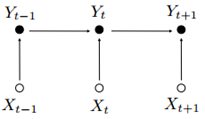
\includegraphics[scale=0.7]{imgs//2-1_Markov_Chain}
    \caption{Markov Chain}
    \label{Markov Chain}
\end{figure}

但是HMM与CRF\cite{lafferty2001conditional}的入手角度不同,HMM是属于生成模型,在计算P(Y|X)时是通过朴素贝叶斯公式通过求得P(X,Y)的联合概率分布求得概率,即P(Y|X)=(P(X,Y))/(∑▒〖P(X,Y)〗)。缺点是当状态转移较复杂时,计算耗时,同时对数据集数量要求较高。CRF\cite{lafferty2001conditional}以及MEMM解决思路是不需要计算X,Y联合概率,而是通过特征函数(拟合得到)直接预测P(Y|X),属于判别式模型。遗憾的是MEMM公式由于局部归一化,所以在求解过程中会出现标注偏置问题(labeling bias),而CRF\cite{lafferty2001conditional}将归一化部分提到了外部,使问题在全局层面上求解。
	
CRF\cite{lafferty2001conditional}的提出更多应用于NLP领域,而将其应用在CV领域时,需要我们把一些前提显式定义,包括图像像无向图的转换,隐状态的转移概率等。\cite{krahenbuhl2011efficient}中提到将图像处理中的先验知识用于能量损失的定义,包括我们趋向于将颜色相近的像素,区域临近的像素识别为同一个类别。而FCN\cite{long2015fully}的输出结果对应P(Y|X)。定义能量函数表达式如图\ref{CRF}。
\begin{figure}[h]
    \centering
    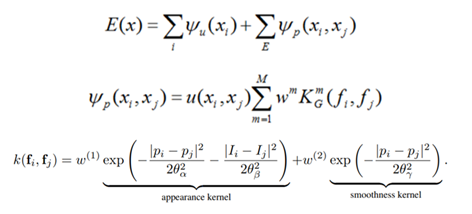
\includegraphics[scale=0.7]{imgs/formula_2-2_function_of_CRF_in_CV.png}
    \caption{CRF loss function}
    \label{CRF}
\end{figure}

目标函数包括两个部分,CFN\cite{long2015fully}的输出和像素点间能量。像素点间能量又由两部分组成,包括颜色相近程度和位置相邻程度,外加一个平滑项。此处使用了全连接条件随机场以从整张图像角度进行判别。

\subsection{强监督学学习}
\label{strong}
前文提到的FCN\cite{long2015fully}模型,在训练时候需要逐像素的计算损失函数。这也就意味着训练的label数据是pixel-level的,而不像物体检测的label是region-level。
	除了FCN\cite{long2015fully}之外,还有很多经典的语义分割模型。
\subsubsection{SegNet}
FCN\cite{long2015fully}中为了将抽象的高层特征图恢复到原图像大小,使用了上采样和越级连接。但是这种粗糙的做法对图像的细节恢复仍然不尽如人意,所以SegNet\cite{badrinarayanan2017segnet}中使用了经典的"编码-解码"结构,同样是通过卷积提取图像特征,但是通过上采样和反卷积进行恢复,同时,考虑到在卷积的过程中,主要的位置丢失发生在池化层,所以SegNet\cite{badrinarayanan2017segnet}在卷积过程中记录下(最大)池化前后的对应位置,在解码阶段,先根据记录的对应位置信息进行上采样,这样得到稀疏的特征图,之后再通过反卷积重建。整体模型结构如图\ref{SegNet}。
\begin{figure}[h]
    \centering
    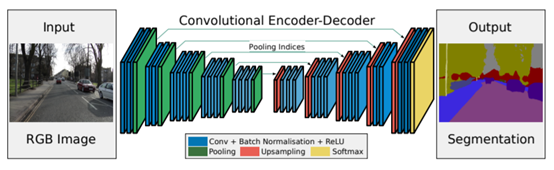
\includegraphics[scale=0.7]{imgs/2-3_SegNet_framework.png}
    \caption{SegNet framework}
    \label{SegNet}
\end{figure}

整个网络模型的编码部分采用VGG16\cite{simonyan2014very}的前13层卷积网络,在解码部分,一个解码器对应一个编码器,以在上采样阶段通过对应的编码器池化时记录的位置信息精确恢复细节。同样的,正如上文提到的,可以在SegNet\cite{badrinarayanan2017segnet}后接CRF\cite{krahenbuhl2011efficient}能将精度小幅提升。

\subsubsection{Deeplab}
Deeplab\cite{chen2014semantic}模型是由Google的团队提出,迭代了4个版本,v1\cite{chen2014semantic},v2\cite{chen2018deeplab},v3\cite{chen2017rethinking},v3+\cite{chen2018encoder}。

Deeplab\cite{chen2014semantic}最早的版本是15年提出,文章指出FCN\cite{long2015fully}模型中存在两个问题,在对图像进行池化下采样的过程中细节信息会丢失,其次,由于卷积所特有的特点,位置信息模糊,所以细节部分的判别不够精细。针对第一个问题,使用空洞卷积来提高感受野,第二个问题通过后接CRF\cite{krahenbuhl2011efficient}进行细节判定。整体的Deeplab\cite{chen2014semantic}网络结构基于VGG16\cite{simonyan2014very}。模型结构与SegNet\cite{badrinarayanan2017segnet}大同小异。

在第二个版本中,Deeplab\cite{chen2018deeplab}在空洞卷积的基础上更进一步,考虑到空洞卷积虽然相较于卷积具有更大的感受野,但是单一大小的空洞卷积核捕获的图像特征较为单一,所以考虑引入ASPP(atrous spatial pyramid pooling),即空洞卷积金字塔,基本思路是在进行卷积时,通过同样大小(3X3),但是rate(r=6,12,18,24)不同的空洞卷积,以捕获不同尺度下的区域特征,之后再将若干个空洞卷积的结果线性相加。同时,16年的时候,随着ResNet\cite{he2016deep}的横空出世,大放异彩。Deeplab也很及时地将其应用,由原来的基于VGG\cite{simonyan2014very}改成了基于ResNet-101\cite{he2016deep}。

在Deeplabv3\cite{chen2017rethinking}中,论文对ASPP做出了改进,同时通过大量的实验论证了ASPP能很好地捕捉不同尺度下的特征信息。对于ASPP的改进,与其说是改进,我认为更多的是对空洞卷积的应用总结。作者设计了两种形式的空洞卷积结构"纵式结构","串联结构"。纵式结构和Deeplabv2大同小异,只是多了个1x1的conv以及全局池化。而串联结构是在网络的每一层只使用一种rate大小的空洞卷积,但是随着网络深度的增加,rate也随之变大。

Deeplabv3+\cite{chen2018encoder}的主要工作不再特征提取阶段,而是在基于特征的恢复阶段。在Deeplabv3\cite{chen2017rethinking}中通过ASPP得到的低分辨率的特征图,是直接通过8倍上采样得到最终的输出,显然这是很暴力粗糙的,所以此处借鉴了"编码-解码"结构,在解码阶段,先上采样4倍,将其与未传入ASPP的low-pixel的语义信息进行拼接后在接反卷积和上采样4倍得到原始图像大小的结果。同时,作者在论文中也对比了以ResNet\cite{he2016deep}和Xception\cite{chollet2017xception}分别作为网络主干的实验效果。Xception\cite{chollet2017xception}效果更胜一筹。

\subsubsection{RefineNet}
RefineNet\cite{lin2017refinenet}在网络结构上与SegNet\cite{badrinarayanan2017segnet}大同小异。文章的出发点在于如何将分辨率较低的特征图恢复至原图像大小,本文的主要工作体现在对"解码"阶段的优化。FCN\cite{long2015fully}的思路是将编码时低维度的信息输入至"解码"阶段,迭代训练得到分辨率高的结果,SegNet\cite{badrinarayanan2017segnet}是通过反卷积将低分辨率的特征图恢复,同时也使用low-pixel的信息作为指导。RefineNet\cite{lin2017refinenet}与SegNet\cite{badrinarayanan2017segnet}的主要区别体现在主干网络的选择与低维信息如何指导"解码"。SegNet\cite{badrinarayanan2017segnet}通过记录池化的位置信息来帮助"解码"执行精确的上采样,而RefineNet\cite{lin2017refinenet}整个网络使用了大量的残差连接,除了网络的主干使用ResNet\cite{he2016deep},将"编码"阶段的卷积结果连至"解码"阶段也是使用残差连接,所以整个RefineNet\cite{lin2017refinenet}中有"short-range"和"long-range" 的connection。图\ref{RefineNet}为RefineNet\cite{lin2017refinenet}的"解码"部分。
\begin{figure}[h]
    \centering
    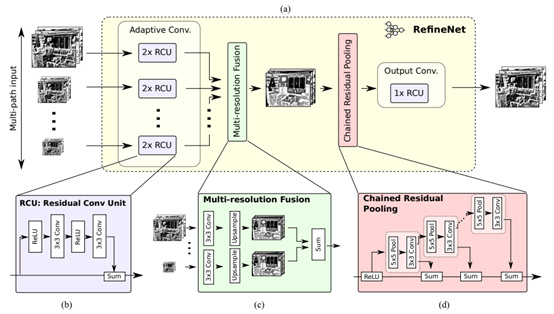
\includegraphics[scale=0.6]{imgs/2-4_components_of_RefineNet.png}
    \caption{components of RefineNet}
    \label{RefineNet}
\end{figure}

\subsubsection{PSPNet}
PSPNet\cite{zhao2017pyramid}在多个数据集上的效果是要好于以上介绍的模型,PSPNet\cite{zhao2017pyramid}的思路是认为FCN\cite{long2015fully}在特征捕捉层面缺乏全局性,即没有很好的上下文关联能力。本文的主要工作是在于特征提取模块的改进,回顾Deeplab\cite{chen2014semantic}的做法,为了在不降低分辨率的情况下捕获更大范围的语义信息,使用了多个不同尺度的空洞卷积。但这样捕获的特征仍然全局性较弱,所以PSPNet\cite{zhao2017pyramid}在池化上做文章,先通过带孔的残差网络ResNet\cite{he2016deep}获得原图像1/8大小的特征图,之后通过不同尺度的池化获得大小为分别为1X1,2X2,3X3,6X6大小的特征图,分别后接1X1的卷积起降维的作用,之后上采样至原图像1/8大小,与前面得到的特征图拼接,这样得到的特征维数增加了,包含了更大尺度的信息。主要部分的结构如图\cite{PSPNet}。
\begin{figure}[h]
    \centering
    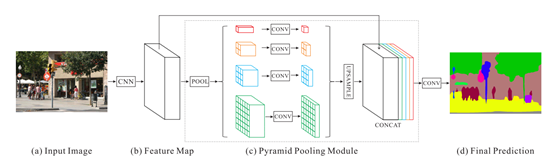
\includegraphics[scale=0.7]{imgs/2-5_Overview_of_PSPNet.png}
    \caption{Overview of PSPNet}
    \label{PSPNet}
\end{figure}

\subsection{弱监督学习}
\label{weakly}
在\cite{strong}中主要介绍了强监督的若干模型方法,在训练时的label是像素级别的标注,但是在实际生活中,像素级的数据集是非常宝贵的,标注成本很高,所以人们将关注点移到如何在精细程度较低的监督下完成语义分割的任务,即弱监督的语义分割学习。弱监督的label没有明确定义,包括:
\begin{itemize}
\item label是图像中存在的物体,图像级别的label,和图像识别的label相同。
\item Label是图像的文字描述,涉及VQA(Visual Question Answer)范畴。
\item Label是图像的Bounding Box,和物体检测的label相同。
\end{itemize}

由于图像级别的label数据集最广泛,成本也最低,所以吸引了大量学者的关注。本部分介绍的模型也只设计图像级别的弱监督学习。

\subsubsection{CAM}
和监督学习语义分割的开山之作FCN\cite{long2015fully}一样。CAM(Class Activation Mapping)\cite{zhou2016learning}是目前大多数弱监督学习的切入角度,CAM\cite{zhou2016learning}主要贡献在于将卷积神经网络的强大在一定程度上进行了可视化,揭示了经过图像识别训练的卷积神经网络在处理新图像时,依然能够将关注重点聚焦至物体所在区域。具体实现细节如图\cite{CAM}。
\begin{figure}[h]
    \centering
    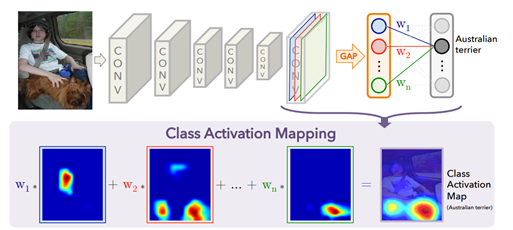
\includegraphics[scale=0.7]{imgs/2-6_Class_Activation_Mapping.png}
    \caption{Class Activation Mapping}
    \label{CAM}
\end{figure}

如图\ref{CAM}所示,首先是经过卷积分类模型,可以使用AlexNet\cite{krizhevsky2012imagenet},VGG\cite{simonyan2014very},GoogLeNet\cite{szegedy2015going}等,之后将其最后的全连接层删去,后接一个卷积层和一个GAP(全局平均池化)得到一个向量输出,接FC层SOFTMAX至输出节点。将此网络进行fine-tuned。训练好后的网络就可以用于物体检测,具体方法是将未传入GAP的特征图与其对应的FC层权重相乘后线性相加。最终就能得到对应探寻物体的热力图。CAM\cite{zhou2016learning}的成功也肯定了卷积在处理图像时仍能很好地保留物体位置信息。

\subsubsection{STC}
STC\cite{wei2017stc}是只基于显著性做出的模型,模型共有3个子模型,呈递进关系。I-DCNN,E-DCNN,P-DCNN。模型结构如图\cite{STC}。
\begin{figure}[h]
    \centering
    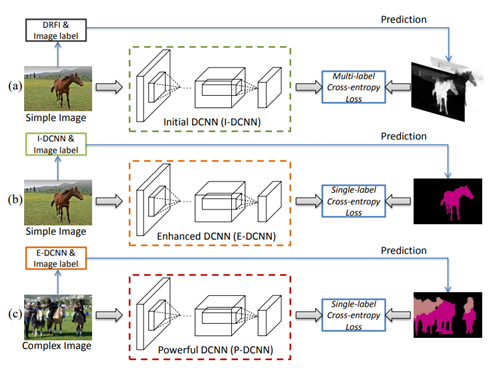
\includegraphics[scale=0.6]{imgs/2-7_(STC)_framework.png}
    \caption{STC framework}
    \label{STC}
\end{figure}

图像的显著性在单物体,背景平滑的图像上效果良好,因此我们受此启发,将简单的图像通过显著性检测方法(DRFI\cite{jiang2013salient})获得图像的显著性区域和背景,并将其作为label对I-DCNN进行训练。训练后的I-DCNN能够输出粗糙的图像语义掩码,我们将I-DCNN的输出结合图像级label进行整合,作为训练E-DCNN的label。E-DCNN经过训练后具有了比I-DCNN更强的分割能力,之后我们让E-DCNN处理复杂的图像,即多标签数据,E-DCNN能获得粗糙的多张语义掩码,同样再次的,将这些掩码与图像级label进行整合,作为训练P-DCNN的label,最终训练好的P-DCNN能够得到较好的图像语义分割结果。

\subsubsection{SEC}
SEC\cite{kolesnikov2016seed}切入角度与STC\cite{wei2017stc}不同,由于CAM\cite{zhou2016learning}的良好定位效果,考虑利用CAM\cite{zhou2016learning}得到的结果综合其他方法获得语义分割结果。SEC\cite{kolesnikov2016seed}的主体框架如图\cite{SEC}。
\begin{figure}[h]
    \centering
    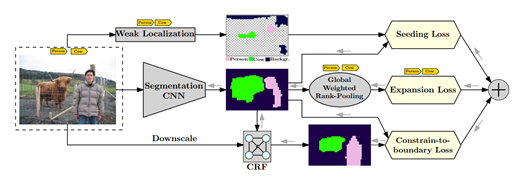
\includegraphics[scale=0.7]{imgs/2-8_framework_of_SEC.png}
    \caption{framework of SEC}
    \label{SEC}
\end{figure}

整体网络由3个loss function组成,Seeding Loss表征预测结果与CAM结果的相符程度,Expansion Loss用于扩展预测区域(CAM的预测结果只聚焦至物体最具辨识度的局部),所以设置Expansion Loss通过使用介于全局池化和平均池化之间的GWAP(Global Weighted Rank Pooling)方式使得获得的物体区域能有所扩展。但是这样扩展的物体区域可能不规整,缺乏良好的边界轮廓,所以此处设置第三个loss用于限制轮廓,与强监督学习中使用CRF\cite{lafferty2001conditional}进行后场处理类似,此处将输出与CRF计算KL散度作为损失函数,以使得模型的边界拟合CRF\cite{lafferty2001conditional}的结果。
	
在性能方面,SEC\cite{kolesnikov2016seed}在多个数据集上的表现效果与STC\cite{wei2017stc}的效果相近。

\subsubsection{AE-PSL}
\begin{figure}[h]
    \centering
    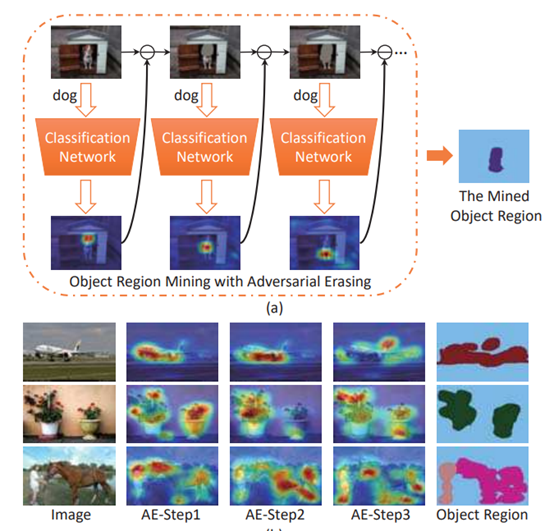
\includegraphics[scale=0.5]{imgs/2-9_AE_approach.png}
    \caption{AE approach}
    \label{AE}
\end{figure}

AE-PSL\cite{wei2017object}是CVPR17的文章,与前面复杂的处理步骤相比,本篇文章以一种很简单直观的方式在弱监督学习下取得了state-of-the-art的效果。

AE-PSL\cite{wei2017object}的思路依然是基于CAM\cite{zhou2016learning},前文提到由于CAM\cite{zhou2016learning}虽然能够反映出CNN在图像上的关注重点,但是容易聚焦到物体最具辨识度的位置,比如动物的头部等局部位置,而语义分割我们更希望得到物体的全部。而CAM\cite{zhou2016learning}之所以聚集在局部是因为物体的某些部位最具有辨识度,在进行判别时作为主要的参考依据。AE-PSL\cite{wei2017object}的思路是强迫卷积神经网络去学习物体的各个位置,具体的设计思路如图\ref{AE}。
AE-PSL\cite{wei2017object}共执行三次CAM\cite{zhou2016learning},第一次可以获得物体的显著局部,如动物的头等,之后我们将对应的图像区域略去,在次进行训练,即强迫CAM\cite{zhou2016learning}去学习属于物体但是辨识度可能没有那么高的区域。经过三次迭代后我们发现基本上物体的整个区域都能被覆盖。但是这样AE得到的结果边界仍然较为粗糙,所以作者又制作了一个PSL网络,网络的损失函数由两部分构成,一部分是AE的结果的相近程度,另一部分是通过对图像进行识别得到的特征图置信度作为特征图的权重相乘后接最大池化得到的结果的相似程度。PSL的引入能将结果的准确率在提升3个百分点。
\begin{figure}[h]
    \centering
    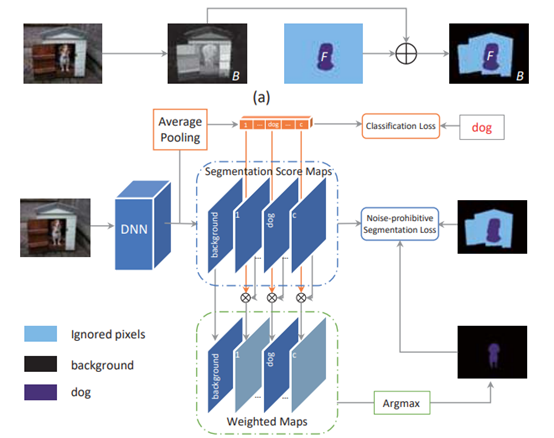
\includegraphics[scale=0.7]{imgs/2-10_PSL_approach.png}
    \caption{PSL approach}
    \label{PSL}
\end{figure}

\subsubsection{AFFNet}
AFFNet\cite{ahn2018learning}是CVPR18的论文,以前面介绍的几篇文章\cite{kolesnikov2016seed,wei2017object}基本思路类似,本文也是two-stage的模型,首先由CAM\cite{zhou2016learning}获得物体的基础轮廓,之后通过图像像素亲和度的关系将CAM\cite{zhou2016learning}粗糙的边界轮廓特征进行完善。基本模型构建如图\ref{AFFNet}。
\begin{figure}[h]
    \centering
    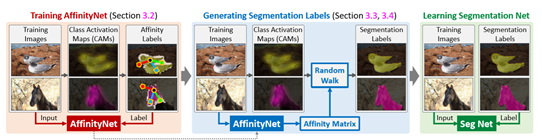
\includegraphics[scale=0.7]{imgs/2-11_process_of_AFFNet.png}
    \caption{process of AFFNet}
    \label{AFFNet}
\end{figure}

如图所示,论文的主要工作在于第二部分,基于CAM\cite{zhou2016learning}的图像分割结果获得任意两像素点之间的相似程度,将其作为之后的AffinityNet的训练label。AffinityNet是一个卷积神经网络,输入一张图像,对于图像上的每个像素点,输出一个描述向量。如果两个像素点属于同一个类,则描述向量越类似。该网络的意义在于帮助CAM\cite{zhou2016learning}中低置信度区域(未归属类的区域)通过像素相似度确定将其归为前景或背景,这样就扩展了初始的较小区域,解决了问题。

\subsection{模型小结}
语义分割的发展不是独立的,随着图像分类,物体检测等领域技术的进步,语义分割的模型也会借鉴其他领域的技巧和解决方式。包括利用残差网络等性能更棒的网络作为backbone,在或者SPP原本应用于物体检测中的思想经过变形用于Deeplab模型中。

强监督语义分割模型目前性能最主要的瓶颈或者说亟待解决的问题有两个,首先是如何使深层卷积神经网络在不损失语义表达的前提下拥有更精确的位置信息,其次是卷积无法适应多尺度的目标,容易导致细小物体的丢失。
对于第一问题,常用的做法是使用CRF作为后场处理以得到精细轮廓,或使用空洞卷积使在不进行下采样的前提下依然能捕获更大范围的上下文信息。

第二个问题的解决思路可以简单归纳为四类。
\begin{itemize}
    \item 图像金字塔,在网络的输入前通过图像缩放显式地改变物体尺度。缺点在于方法较耗时而且很不优雅。
    \item 编码-解码结构,在解码阶段通过对应编码阶段的信息辅助恢复图像。代表模型是U-net\cite{ronneberger2015u},SegNet\cite{badrinarayanan2017segnet}。
    \item 空洞卷积,在不同的卷积层使用不同大小的空洞卷积,就能捕获不同尺度下的信息。而且空洞卷积的引入也有助于解决第一个问题,所以在之后的Deeplab\cite{chen2014semantic}版本中取消了CRF\cite{lafferty2001conditional}后场处理。
    \item 空间金字塔池化,由于卷积阶段捕获的特征主要在小区域范围,所以SPP通过将全局进行不同尺度的池化作为全局信息补充。与图像金字塔的区别在于是特征图层面的金字塔。代表模型是PSPNet\cite{zhao2017pyramid}。
\end{itemize}

除了以上介绍的模型,还有很多优秀的强监督语义分割模型,如FRRN\cite{pohlen2017full},ICNet\cite{zhao2018icnet},Dilation10\cite{yu2015multi},以及基于PSPNet改进的ESPNet\cite{mehta2018espnet}等。
弱监督语义分割的发展其实一直没有实质性的性能突破,目前最主流的算法框架可以拆分为两个部分。
\begin{enumerate}
    \item 基于CAM\cite{zhou2016learning}获得先验物体区域。部分学者在CAM\cite{zhou2016learning}模型上进行改进,如更换网络主体,通过擦除等获得更棒的区域效果。
    \item 经过CAM\cite{zhou2016learning}处理后的图像中仍然存在前景和背景置信度都较低的待定区域,所以学者通过结合其他图像处理手段,如物体显著性检测,亲和度网络,种子随机游走等对待定区域进行判别分割归属。
\end{enumerate}

之后可以通过CRF等进一步进行完善。目前弱监督语义分割的识别准确率与强监督语义分割模型在PASCAL VOC 2012上的测试集mIoU指标上仍有接近30个百分点的差距。其他一些优秀的模型包括MIL-FCN\cite{pathak2014fully},CCNN\cite{pathak2015constrained},DCSM\cite{shimoda2016distinct}等。

\section{评测数据}
由于语义分割的数据集成本较大,所以常见的语义分割数据集较少,主要包括: PASCAL VOC 2012\cite{pascal-voc-2012},Cityscapes,CamVid\cite{brostow2008segmentation,brostow2009semantic},Stanford Background\cite{liu2010single,saxena2006learning,saxena2007learning}等。其中最常用的是PASCAL VOC 2012,所以评测数据部分以介绍此数据集为主。

PASCAL VOC 2012:该数据集主要的贡献者是来自欧洲包括牛津,剑桥,苏黎世理工等学校的学者。数据集从2005年最初只有四个类别开始,经过不断地发展更新,到2012年数据集已经具有一定规模了,之后没有继续迭代,沿用至今。

正如名字所述(visual object classes)。其涵盖范围包括:分类/检测图像数据,分割图像数据,动作分类图像数据,人体姿态图像数据等。本文讨论语义分割,所以此处介绍分割图像数据。

\begin{itemize}
    \item PASCAL VOC 2012:用于语义分割的图像包括20个类,分别是(1=aeroplane, 2=bicycle, 3=bird, 4=boat, 5=bottle, 6=bus, 7=car , 8=cat, 9=chair, 10=cow, 11=diningtable, 12=dog, 13=horse, 14=motorbike, 15=person, 16=potted plant, 17=sheep, 18=sofa, 19=train, 20=tv/monitor)。而在是实际运用中,我们还会多设置一个类为背景,对应数据集label中数值为0的黑色区域。示例如图\ref{VOC example}。
\begin{figure}
    \centering
    \subfigure[original]{
        \begin{minipage}[t]{0.4\linewidth}
        \centering
        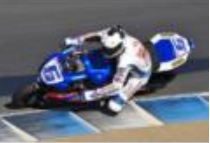
\includegraphics[width=1in]{imgs/3-1_left_original.png}
        \end{minipage}
    }
    \subfigure[label]{
        \begin{minipage}[t]{0.4\linewidth}
        \centering
        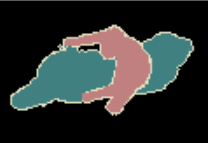
\includegraphics[width=1in]{imgs/3-1_right_segmentation_label.png}
        \end{minipage}
    }
    
    \caption{ample in PASCAL VOC 2012}
    \label{VOC example}
\end{figure}

数据集中训练集和测试集以及验证集的数量如图\ref{VOC statistic}
\begin{figure}[h]
    \centering
    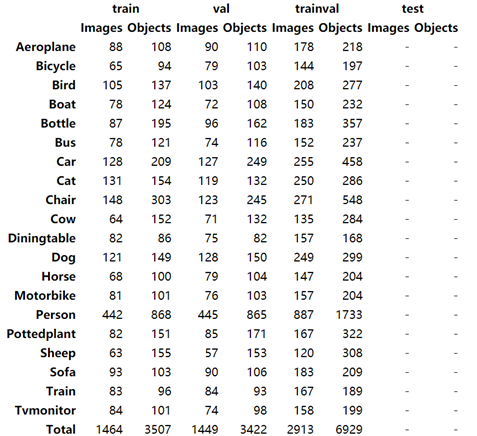
\includegraphics[scale=0.7]{imgs/3-2_VOC_2012_statistic.png}
    \caption{PASCAL VOC 2012 图像数量统计}
    \label{VOC statistic}
\end{figure}
训练集和验证集的数量大致相当,而且两者的物体数量分布也大致相等。

    \item Cityscapes:是取自50个城市,不同季节,不同时间,不同天气的成熟景象。收录了5k张的精细图像和2w张略粗糙图像,收录了30个类。
    \item CamVid:全称为 Cambridge-driving Labeled Video Database。是第一个将视频制成语义标准的数据集。拥有32个道路常见的类,包括树,墙,天空,小孩子等。
    \item Stanford Background:是一个小型的数据集,主题是户外。每张图像大约320X240像素大小,收录了7个类,包括400张训练集和134张验证集。
\end{itemize}


\section{评测手段}
对模型的好坏判别一般有两方面,模型计算性能,模型计算速度。主要的考察标准以性能为主,但是在一些对实时性要求较高的情形,如无人驾驶等需要对计算速度有一定要求。
\begin{itemize}
    \item 计算性能:主要评价指标为mIoU(mean intersection over Union)的缩写,翻译汉语是平均交并比。对于一张图像,我们经过网络模型得到了一张分割图,图中的每个点都属于某个前景或者背景,那么我们将输出分割图与label图像进行交并运算,得到结果。以识别图像$I$中的汽车$C$为例,对于模型输出,判定为汽车的像素集为$S_{out}$,而该图像I中汽车真实的像素集为$S_{label}$,则对于$I$和$C$,此时的IoU为$\frac{S_{out}\cap S_{label}}{S_{out}\cup S_{label}}$。而mIoU就是遍历每个$I$,每个$C$,通过面积大小进行加权平均得到模型对某个数据集的mIoU指标,通常我们会对照模型在验证集和测试集上的效果。
    \begin{figure}[h]
    \centering
    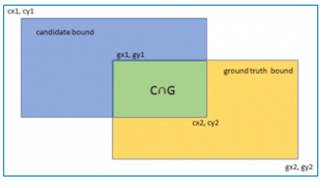
\includegraphics[scale=0.8]{imgs/3-3_IoU.png}
    \caption{PASCAL VOC 2012 图像数量统计}
    \label{VOC statistic}
\end{figure}
    \item 速度性能:参考的指标为模型从输入图像到输出分割结果的速度,单位通过以帧率(fps)为准,当然由于运算平台的差异,模型运算速度也有所不同,所以学者通常会将测试平台,包括GPU型号,数量等作交代。
\end{itemize}

\section{开放问题}
目前的语义分割仍然处在发展期,跟随着CV领域其他方向共同进步。目前在PASCAL VOC上强监督学习的模型mIoU指标能达到90-\%。而弱监督(image level)的mIoU指标达到60+\%。这仅仅是20个类别的情况下。所以我认为目前强监督模型的发展已经达到较高水准,而主要的限制瓶颈在于提升运算水平和如何处理更多类别。而弱监督模型目前的准确率仍然处于偏低,如何进一步提升模型能力可能需要进一步挖掘卷积的潜力等。

\section{结论}
语义分割相较于物体(目标)检测,更加的符合人类视觉,所以研究语义分割更有助于挖掘神经网络与人脑处理视觉信息的相似性。目前神经网络的可解释性仍然有待进一步发展,纵观神经网络的发展历程,从最初始的全连接层,受局部相关性的启发,卷积神经网络大放异彩,在节省参数的前提下提升了性能,在到之后CAM\cite{zhou2016learning}进一步挖掘了卷积神经网络具有的定位能力,这也是弱监督的基础。同时,残差网络,Inception,Xception,BN\cite{ioffe2015batch}等general的优化思路也帮助语义分割模型性能更进一步。

但是和其他神经网络相关的领域的所面临的问题一样,神经网络的可解释性依然不够,只有更好的理解神经网络,才能更好更精确的预测输出结果,从而改进网络。













\bibliographystyle{plain}
\bibliography{references}
\end{CJK}
\end{document}